\chapter{Introductory Material}
\label{Introduction}
% discuss SPECT and Multimodal 
% SPECT 
% Photon Detection (and collimation)
% Event reconstruction .Recon techniques pg51 Mic.
%Image Recon 
% Calibration Techniques Deb Pg. 49 

This thesis outlines the evaluation of a \acrshort{SPECT} imaging system, designed for the simultaneous use within a clinical \acrshort{MRI} system. This chapter outlines the basics of \acrshort{SPECT} imaging systems, discusses the use of multi-modality imaging and introduces the novel combined imaging system; the \acrshort{INSERT} scanner. 

\section{SPECT}
The \acrlong{SPECT} system was introduced by \cite{Anger1958ScintillationCamera} as a method of retrieving a signal from the detection of gamma photons. \acrshort{SPECT} is used widely as a medical imaging technology to investigate the physiological response of an injected radio-pharmaceutical. A pharmaceutical is chosen by its ability to target a given biological process or organ, this drug is labelled with a gamma emitter \cite{Chiewitz1935Radioactive1}. The localised emission is detected by the \acrshort{SPECT} camera and the resulting signal is reconstructed into a 3D tomographic image. The main components of the \acrshort{SPECT} developed by \cite{Anger1952UseStudies} are the collimator, scintillation crystals and \acrlong{PMT}. The gamma rays emitted from the patient will travel toward the camera head; they interact with the scintillation crystal producing a light pulse, the \acrshort{PMT} will amplify this pulse and convert it to an electrical signal for processing. The signals are processed using Anger logic, \cite{Peterson2011SPECTBeyond.}, however without a geometric context it is impossible to localise the origin of the gamma ray; the collimator acts as a camera aperture by allowing only gamma rays from a chosen direction to enter the crystal.

Photon detection within a \acrshort{SPECT} is governed by many factors. The collimator design is the largest contribution to sensitivity, resolution and \acrlong{FOV} of the system \cite{0031-9155-50-21-004}. The choice of collimator must consider a balance between number of photons detected and the quality of localisation. A high resolution will improve localisation but is achieved by reducing the aperture size; reducing the sensitivity and requiring a longer scanning time \cite{doi:10.1001/jama.1965.03080190014004}. The collimator is also chosen with consideration of the desired image; for example collimator designs such as the pinhole are more suited to small organ imaging \cite{1076033}. The geometry of the collimator determines how the acquired signal is processed into a final image. The chosen collimator geometry defines the photon path however there are uncertainties to consider such as photons penetrating through the collimator septa \cite{Accorsi2008DerivationCollimation} \cite{0031-9155-18-6-005}. 

The localisation of photons is also determined by the design of the scintillation crystals and \acrshort{PMT}. These components determine performance factors of the detector including efficiency, count rate, spatial and energy resolutions, uniformity, and linearity \cite{Anger1966SensitivityCamera} \cite{Sorenson1987}. The size, position and density of the crystal determines the efficiency of photon detection. A greater efficiency improves the count rate as event are not lost in between scintillation interactions due to dead time. The energy resolution is the detectors ability to distinguish the photopeaks within a spectra. The spatial resolution of a detector defines the quality of spatial information for each event, this is governed by the \acrshort{PMT} geometry and the photons \acrlong{DOI} within the crystal \cite{Morrocchi2017}. Uniformity and linearity are important factors in image quality as the spatial response may be unstable depending on time or location \cite{LyraGeorgosopoulouRoutineInstrumentation}.

\section{SPECT Imaging} % Reword
\acrshort{SPECT} imaging systems determine the location of a radioactive tracer within the body from the forward projection of the acquired data \cite{BasicOfNM}. The process of imaging is governed by the solution of the equation \ref{eqn:imgRec}. The value of $x$, the tracer activity, is determined from the acquired data, $Y$, and the system matrix, $S$; subject to a noise term, $\eta$. The solution give a complete image of the object by acquiring projections from several angles. More information from the object is acquired with each addition projection angle. We extract the tracer information from a sinogram; a representation of projection data moving through all covered angles. The reconstructed images are produced through the analytical or iterative solution of \ref{eqn:imgRec}. The projections are created using event reconstruction algorithms. These are based on Anger logic; this thesis focuses on two methods of event reconstruction used to evaluate the projection data acquired from each experiment.

\begin{equation} \label{eqn:imgRec}
        Y = S(X) + \eta 
\end{equation}

\subsection{Event Reconstruction: Centroid Method}
The \acrlong{COM} method, also known as the Centroid method, is a simple reconstruction originating in the first Anger cameras. From Anger logic we know the signal from a scintillation event will decrease further from the interaction point. The Centroid algorithm makes use of this by simply considering a weighted mean of the signal of a given event from each photodetector. 

\begin{equation} \label{eqn:Centroid}
        X_{i} = \frac{\sum^{N}_{j} x_{j} \cdot S_{ij}}{\sum^{N}_{j} S_{ij}} \quad ; \quad  Y_{j} = \frac{\sum^{N}_{j} y_{j} \cdot S_{ij}}{\sum^{N}_{i} S_{ij}}
\end{equation}

The equation \ref{eqn:Centroid} describes the reconstructed event positions $X\_i$ and $Y\_i$ for each event i. The signal $S\_{ij}$ from a given event is summed over each  photodetector j. This weighted sum gives the likely position of an event as the coordinates is calculated toward the centre of the nearest photodetector, $x\_j$ and $y\_j$. The centroid method is modified to account for the event compression towards the centre of a given detector; this modified centroid method subtracts a common baseline, B, value from each event. The baseline subtraction removes signal not within the region of interest and is chosen based on the detectors field of view (\ref{eqn:ModCent}). 

\begin{equation} \label{eqn:ModCent}
        X_{i} = \frac{\sum^{N}_{j} x_{j} \cdot (S_{ij} - B)}{\sum^{N}_{j} S_{ij}} \quad ; \quad  Y_{j} = \frac{\sum^{N}_{j} y_{j} \cdot (S_{ij} - B)}{\sum^{N}_{i} S_{ij}}
\end{equation}

This method is popular as is provides fast and simple projection data. Although the baseline solves the central compression, the centroid method is subject to several errors. 

Non-uniformity in a given camera will distort the resulting projection. Uniformity and sensitivity are subject to the detector response to relative gain and energy window selection. The difference between photodetectors gain can result in false density distribution across the whole detector. The centroid method is unable to account for this as signal will be heavily weighted by a non-uniform photodetector. 

Linearity of the projection data is subject to spatial distortion within the crystal, the centroid method assumes a constant response throughout the crystal. Although true for the centre of the crystal this assumption results in non-linearity at the detector edges. The result is similar to the central compression from equation \ref{eqn:Centroid}.

These issues can be resolved with correction maps and calibration \cite{Miller2012AImagers} \cite{Jin1995CalibrationsMcSPECT-II} as we will see in the following chapters. However we can improve the event reconstruction through statistical methods and spatial modelling \cite{Morozov2015IterativeCamera}. 

\subsection{Event Reconstruction: Maximum Likelihood}
A statistical method of event reconstruction is able  to produce higher quality projection data which is less susceptible to spatial distortions. The \acrlong{ML} algorithm achieves this by accounting for the random nature of gamma particle interactions and extracting probability models from acquired data \cite{4307558} \cite{JinhunJoung2000ImplementationCameras}.

The \acrshort{ML} algorithm makes use of optical models and the detectors spatial response to calculate the events coordinates and energy. The algorithm optimises a set of model parameters in order to maximise the probability of observing the acquired data from the given model. If we consider our observed data by vector $\Bar{\nu}$, each value is given by detector response to a scintillation event, i.e. number of detected photons or electrical signal, by each channel. The observed data is a result of a series of random events, $V\_i$ (in SPECT imaging this is the transport of gamma rays). The events can be represented by a known probability model, $M(\theta)$, where $\theta$ is the set of optimising parameters. Thus the probability of observing our acquired data given $\theta$ is the joint probability of each independent event $V\_i$ for N total events. 

\begin{equation} \label{eqn:MLProb}
                P(\Bar{\nu}|\theta) = \prod^{N}_{i=i}P(V_i)
\end{equation}

The likelihood of the observed sample, $L(\theta|\Bar{\nu}) = P(\Bar{\nu}|\theta)$, can be maximised to retrieve the unknown parameter which gives the observed data. The standard form for the \acrshort{ML} algorithm takes the log of the maximisation to turn the product into a sum. 

\begin{equation} \label{eqn:ML}
                \hat{\theta} = max\{\sum^{N}_{i=i}log(L(\theta|\Bar{\nu}))\}
\end{equation}


\subsection{Image Reconstruction}
Once the projection data has been reconstructed the final images can be produced from the solution to equation \ref{eqn:imgRec}. Here we briefly describe the iterative approach which is used throughout this thesis. The \acrlong{MLEM} algorithm aims to produce a image model which accounts for the physical interactions involved in \acrshort{SPECT} imaging; optimising the model until it matches the acquired data, \cite{4307558}. Using the \acrshort{ML} logic described above the algorithm carries out a series of forwards and back projections in order to improve a estimated model. The algorithm is composed of two main steps; the estimation stage, and the maximisation stage. The initial estimation can be a uniform image or can be retrieved from a simple back projection of the acquisition data. The estimated model is forward projected to produce a model of the measured projection data. The projection models are then compared with the acquired data. A correction term is derived from this comparison; using the maximum likelihood technique a correction is determined and used to improve out estimation. This is the maximisation step, the result is an improved image when back projection is carried on on the estimation. However this improvement is incremental and so the steps must be repeated; improving the model and creating a image closer to the true object with each iteration.  

\section{Clinical SPECT}
Brian spect and its uses cite cite cite 

\section{Multi-modal Imaging} % dont discuss INSERT 
% Multi modal 
The capabilities of medical imaging continues to improve and expand, however in recent years it has become possible to combine medical imaging systems \cite{PATTON2009247}. Multimodal imaging technologies have gained popularity within research and clinical practice for their ability to simultaneously or sequentially acquire data from multiple systems. Individual systems can provide either functional or structural information, however many patients require multiple scans for diagnosis or treatment. The combination of this information is essential in investigations and can be achieved through methods such as spatial and time registration. However, acquiring multiple scans and registering the images takes many hours and is subject to errors such motion. Multimodal systems can solve this by acquiring both structural and functional information within one simultaneous scan, reducing scan time and improving image registration. 

Introducing the strengths from one imaging system can solve issues present in another. \acrlong{CT} is a well established structural imaging technique. This imaging technique is popular due to its good spatial resolution and short acquisition time. Although favoured for bone imaging, it is capable of imaging software tissue through the use of contrast agents. \acrshort{CT} is able to incorporate attenuation information within reconstructions, this correction is particularly useful in nuclear medicine. The radiation in \acrshort{SPECT} and \acrshort{PET} is subject to attenuation in intensity is lost as the photons travel through matter. The combination of \acrshort{CT} with nuclear medicine provides an attenuation correction which can improve image quality at a lower dose \cite{Blankespoor1996AttenuationAssessment}. Multimodal \acrshort{SPECT/CT} and \acrshort{PET/CT} have become well established as the imaging systems are easily integrated in both sequential and simultaneous systems \cite{Schillaci2005HybridImaging}.

\acrshort{MRI} is a multifaceted imaging technique which provides a greater soft tissue imaging and is not limited to structural imaging. The use of magnetic fields and radio frequency provides no ionising dose to the patient. For these reasons it can favourable to \acrshort{CT}, especially in the monitoring and stratification of cancer treatment, where minimal dose is a priority \cite{Cherry2009MultimodalitySPECT/CT}. Recent work looks to establish attenuation correction through \acrshort{MRI}, fulfilling the role of \acrshort{CT} \cite{Zaidi2007IsImaging},\cite{Hofmann2008MRI-basedRegistration}. However due to the strong magnetic fields, \acrshort{MRI} is difficult to combine with other imaging systems. Ferrous metals, motors and electrical or \acrshort{RF} noise can prevent the \acrshort{MRI} from functioning. To obtain the advantages of combined \acrshort{MRI} with nuclear medicine the challenge of achieving mutual compatibility was met. Through the redesign of the photodetectors, \acrshort{PET/MR} was established \cite{PICHLER2008199} \cite{Herbert2004FirstPhotomultiplier}. The standard \acrshort{PMT} used in gamma cameras were unable to work within a magnetic field, advances in solid state detectors which were compatible within \acrshort{MR} lead to the development of the first \acrshort{PET/MR} \cite{0031-9155-56-23-014}. Since its creation \acrshort{PET/MR} has become a powerful imaging system within research and the clinic. 

However a simultaneous \acrshort{SPECT/MRI} clinical system has yet to be established. The combination of \acrshort{SPECT} and \acrshort{MRI} can be carried out through sequential use of \acrshort{SPECT/CT} and \acrshort{MRI}. The data are registered to provide the \acrshort{SPECT/MR} images. The development of simultaneous and integrated \acrshort{SPECT/MRI} promises the advantages of \acrshort{PET/MR}, without the additional dose of a \acrshort{CT} scan \cite{en2019ImageStudy}. \acrshort{SPECT} imaging is more widely available and cheaper than \acrshort{PET} systems; making it popular as it allows the use of more accessible radionuclides and dual-isotope imaging \cite{deRosales2014PotentialAgents} \cite{Bateman2012AdvantagesPractice}. The development of \acrshort{MR} compatibly photodetector has not yet lead to clinical \acrshort{SPECT/MRI} as \acrshort{SPECT} introduces further complications with compatibility. Many preclinical system however have achieved simultaneous \acrshort{SPECT/MR} \cite{Meng2007DesignImaging}.

The preclinical designs for \acrshort{SPECT/MR} demonstrate feasibility of a \acrshort{SPECT} insert within a clinical \acrshort{MRI} \cite{Cai2014MRC-SPECT:Animals}. Compatibility is achieved in these designed through a stationary scanner design comprised of multiple scanner heads in a ring formation \citer{Tsui2011HighAnimals}. A rotating phantom can be scanned with a single detector head to achieve the same effect \cite{Hamamura2010DevelopmentAcquisition.}. The camera heads make use of \acrshort{MR} insensitive scintillation or semiconductor detectors similar to that of \acrshort{PET/MR}. Developments in \acrshort{CZT} detectors has lead to more preclinical\acrshort{SPECT/MR} systems which aim to upscale components into a clinical design \cite{0031-9155-55-6-002} \cite{Tan2011ExperimentalField} \cite{Cai2013HybridSystem}. The challenge of developing a collimator has been tackled in several ways. Many designs favour a multi-pinhole collimator to provide the compact design requirements without loss of \acrshort{FOV} \cite{Meier2011AAnimals}. These designs are composed of insulated layers or tungsten or tungsten powder to ensure no ferrous material interference. The success of these simultaneous \acrshort{SPECT/MRI} demonstrate its potential applications in tumour treatment stratification and the therapeutics delivery. 

It stands to reason that a simultaneous clinical \acrshort{SPECT/MR} system could provide a multifaceted imaging tool within the clinic. This thesis outlines the use of the\acrshort{INSERT} scanner; the first clinical simultaneous \acrshort{SPECT/MRI} imaging system. The goal of which is to provide brain tumour imaging and treatment stratification, and establish a foundation of a completely integrated \acrshort{SPECT/MRI} system. 

\begin{figure}[!t]
%\vspace{-0.2cm}
\centering
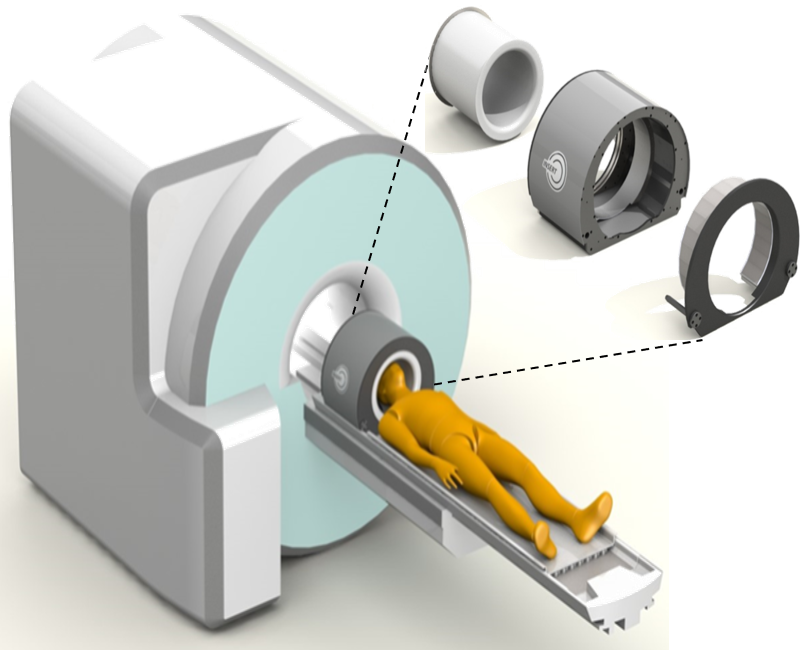
\includegraphics[width=3.6in]{figures/INSERT_clinical.png}

\caption{Complete clinical set up for the \acrshort{INSERT} system.}
\label{fig_INSERT}
%\vspace{-0.2cm}
\end{figure}
